%!TEX program = xelatex
\documentclass[a4paper]{article}

\usepackage[left=3cm,right=3cm,top=3cm,bottom=3cm]{geometry}  % 设置页边距
\usepackage{mathrsfs}  % 数学公式的工具包
\usepackage{graphicx} % 图片加载宏包
\usepackage{subfigure} % 图片并列
\graphicspath{{./}{./figures/}} % 图片加载路径
\usepackage[UTF8]{ctex} % 中文支持
\usepackage{hyperref}
\usepackage{multirow}

\renewcommand{\contentsname}{\centerline{\textbf{\huge{目录}}}}
\newcommand{\titlefont}{\fontsize{36pt}{36pt}\selectfont}
\renewcommand{\normalsize}{\fontsize{14pt}{\baselineskip}\selectfont}

\begin{document}

\begin{titlepage}

	\begin{center}
	
		\null 
		
		\vspace*{7cm}
		
		\hrule
		\vspace*{0.5cm}
		{\titlefont{\textbf{论文研讨报告}}} 
		
		\vspace*{0.5cm}
		\begin{minipage}{0.5\textwidth}
			\begin{flushleft}
				on \textit{Image Style Transfer Using Convolutional Neural Networks \footnotemark }
			\end{flushleft}
		\end{minipage}
		\vspace*{0.5cm}
		\hrule
		
		\vspace*{6cm}
		
		\begin{minipage}{0.5\textwidth}
			\begin{flushleft}
			{\Large{
				\emph{姓名:} qiaoin \\
				\emph{学号:} 20161226 \\
				\emph{学院:} \textit{Computer science} \\
				\emph{完成日期:} \today \\ }} 
			\end{flushleft}
		\end{minipage}
	
	\end{center}
	
	\footnotetext{Gatys L A, Ecker A S, Bethge M. Image style transfer using convolutional neural networks[C]//Proceedings of the IEEE Conference on Computer Vision and Pattern Recognition. 2016: 2414-2423.}
	
\end{titlepage}

\newpage
\clearpage
\tableofcontents 
\thispagestyle{empty}
\newpage

\setcounter{page}{1}

% 从这里开始插入正文即可

\section{第零章}

我们身处大数据时代,每分每秒都伴随有数据产生,在这过去的一分钟里,社交网络平台中发生了什么呢?图 \ref{fig:1} 向我们解释了我们每分钟在网络世界创造了哪些数据\footnote{https://www.domo.com/blog/data-never-sleeps-4-0/} 。但即使是在大数据时代的背景下,我们所存储的近 40\% 文件是小文件和元数据(small files and metadata),大小一般小于4K。

\begin{figure}[!htb]
\begin{center}
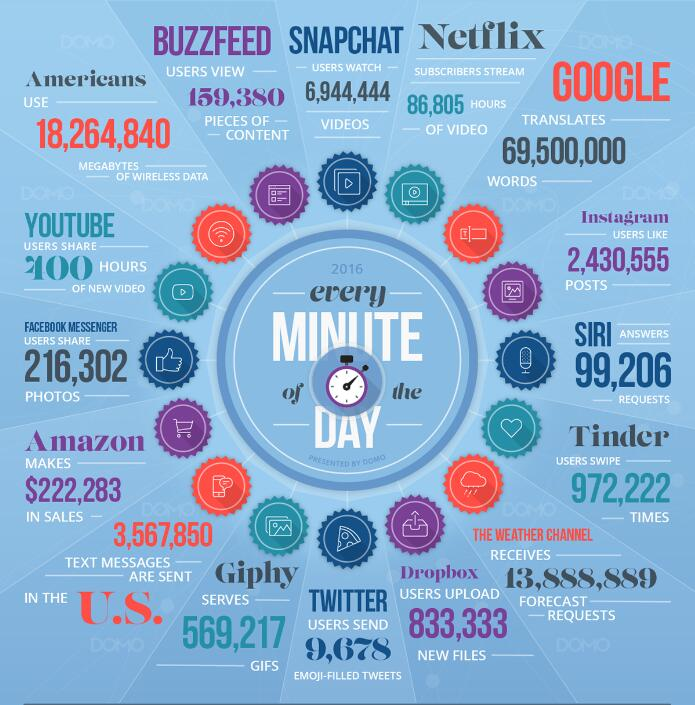
\includegraphics[width=.6\textwidth]{dada_generated_every_minute.jpg}
\caption{大数据时代,一分钟有多少数据产生?} \label{fig:1} 
\end{center}
\end{figure}


\section{第一章}

\subsection{第一章子标题}

\begin{figure}[!htb]
\begin{center}
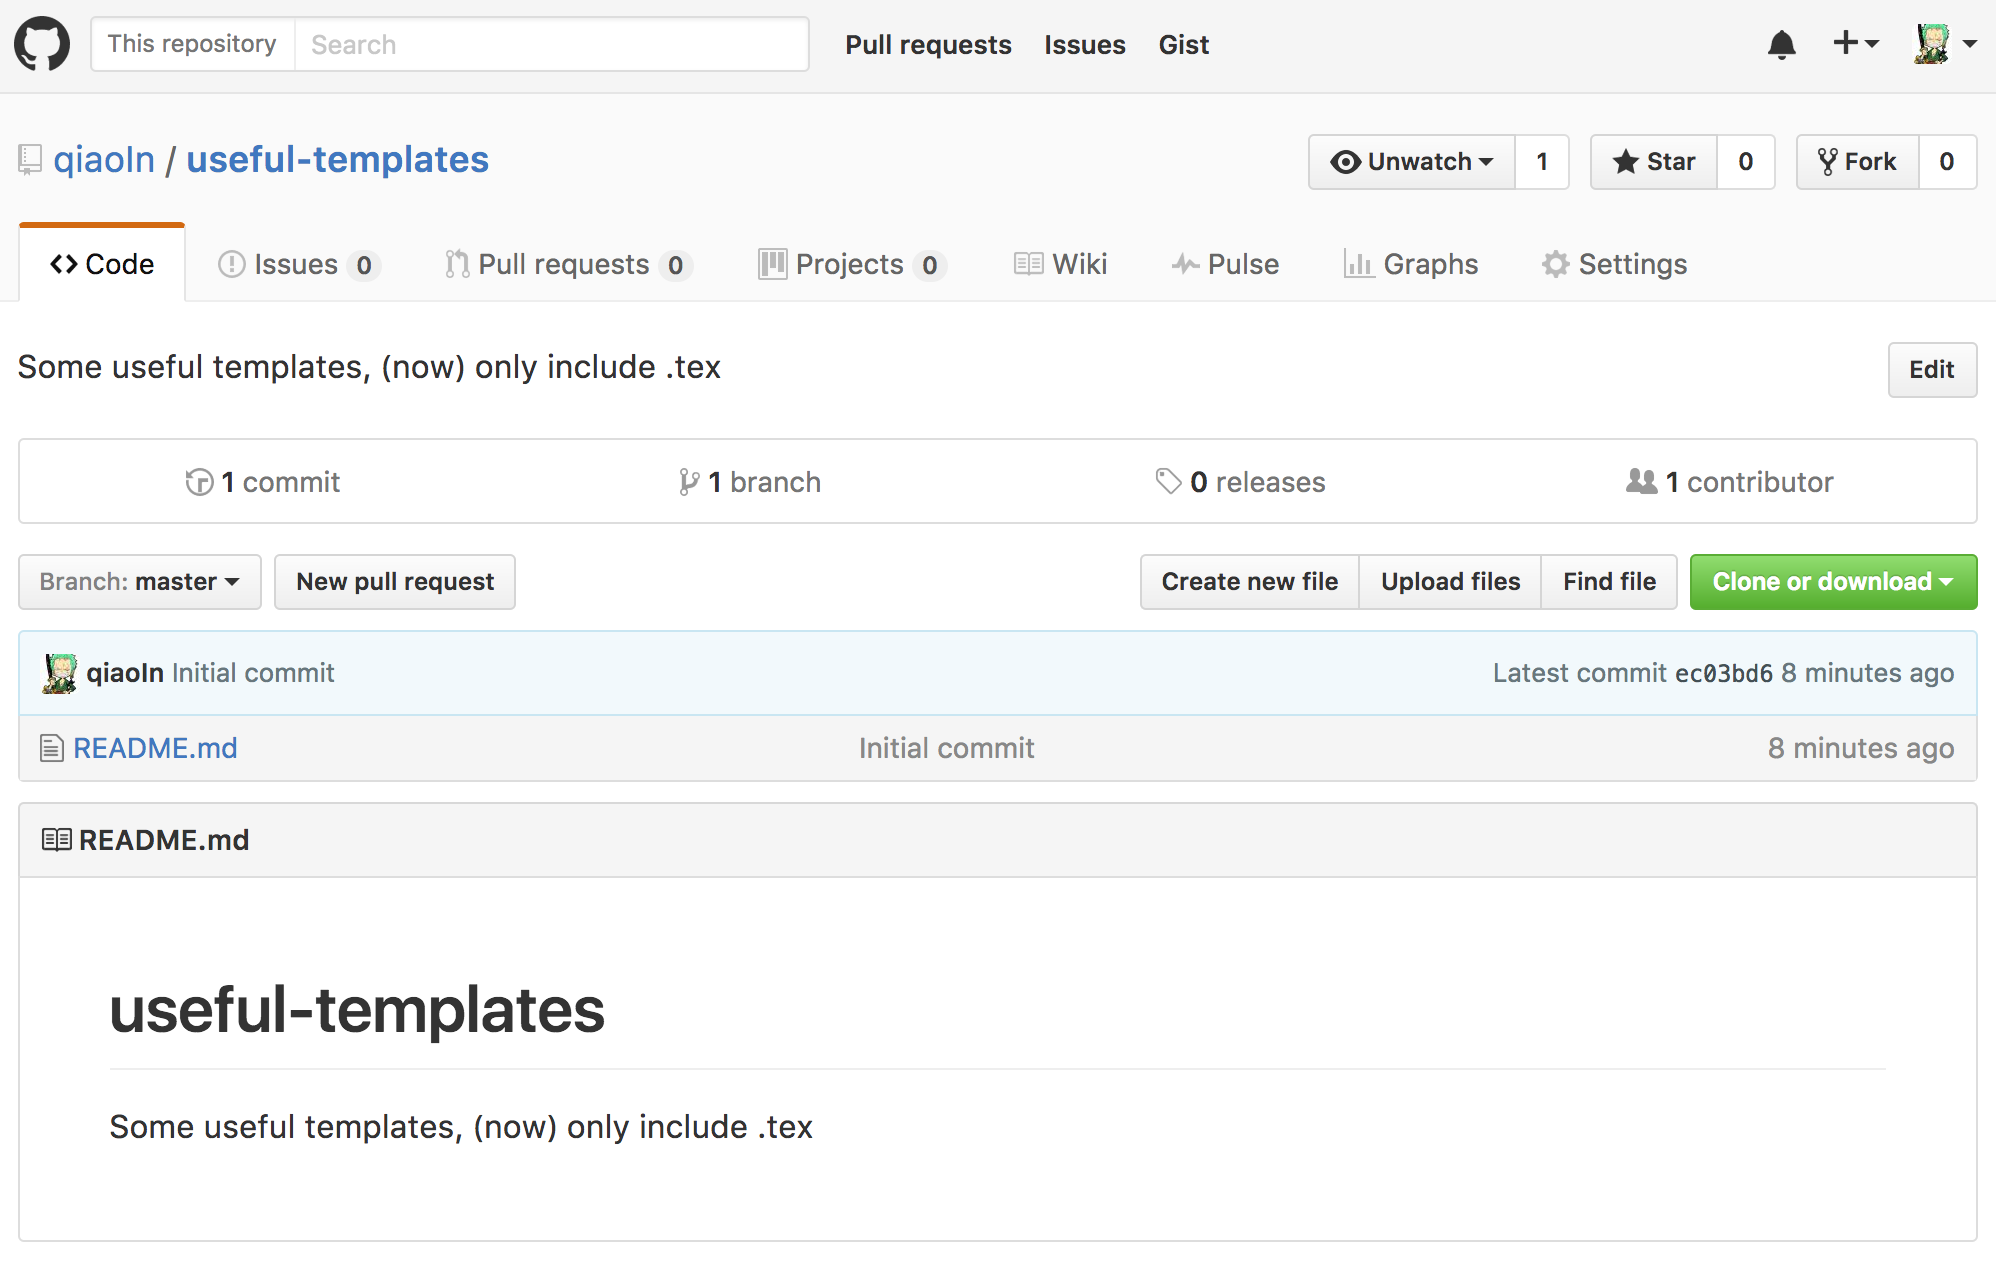
\includegraphics[width=0.85\textwidth]{useful-templates.png}
\caption{repository on Github - useful-templates} \label{fig:3} 
\end{center}
\end{figure}

\subsection{第一章子标题} \label{section-2.2}

列表:
\begin{enumerate}
	\renewcommand{\labelenumi}{\theenumi)}
	\setlength{\parsep}{0pt}
	\setlength{\itemsep}{0pt}
	\item 这是一个列表;
	\item 这仍然是列表的一个条目。
\end{enumerate}

\subsection{第一章子标题}

在这里添加即可。


\section{第二章}

如何制作表格

实验中所用到 Linux 桌面电脑脑配置如表 \ref{tab:1}。
\begin{table}[!htb]
    \centering
        \begin{tabular}{|l|l|} \hline
		Linux				&		Ubuntu 12.10, Kernel 3.6.6 64-bit version \\ \hline
		CPU 				& 	AMD Opteron Processor 242 Dual COre \\ \hline
		DRAM 			& 	16GB DDR SDRAM  \\ \hline
		\multirow{3}{*}{Hard Disk}	
								& 	Western Digital 72ooRPM 2TB STAT Disks \\
								&  	random seeks: 100 seeks/sec peak \\
								& 	sequential reads/writes: 137MB/sec peak \\ \hline
		\multirow{3}{*}{SSD}				
								&  	Intel 2.5-in 128GB 520 Solid State Drive \\ 
								& 	random read 15000 IO/sec, write 3500 IO/sec \\
								& 	sequential read 245 MB/sec, write 107 MB/sec \\ \hline
	   \end{tabular}
    \caption{Linux 桌面电脑配置详细}\label{tab:1}
\end{table}

\subsection{第二章子标题}



\subsection{第二章子标题}


\section{第N-1章}

总结与讨论

\end{document}
















